%%Cp plots

In this section, we focus on $C_p$ for the different meshes considered due to zonal-based refinement/adaptation.
Here, phase averaged and spanwise averaged data is considered over multiple cycles.

A comparison of $C_p$ for the different meshes is shown in Figure \ref{fig:zonal_Cp_plots_LEV}, for four phases of interest leading up to the LEV formation. 
For phase $\psi=150^\circ$, flow has started to separate for Mza2 and Mza3 meshes around $x/c = 0.2$, whereas M0 and Mza1 meshes fail to capture this flow separation. 
Mza2 and Mza3 meshes agree well with each other. 
Note that meshes with same in-plane resolution do not show significant variations with changes in spanwise resolution.

 
For phase $\psi=180^\circ$, M0 mesh does not capture any peak in $C_p$.
Mza1, Mza2, and Mza3 meshes show boundary layer/vorticity roll-up with a peak in $C_p$ around $x/c = 0.1$.
Mza1 meshes shows a lower peak in $C_p$ than Mza2 and Mza3 meshes. 
Flow separation is also not clearly visible in spanwise vorticity plots for Mza1 meshes shown in Figure \ref{fig:vorticity_zonal_180}, as compared to Mza2 and Mza3 meshes.
Mza2 and Mza3 meshes which agree well with each other.


For phase $\psi=210^\circ$, all meshes show LEV formation apart from M0 mesh. Note that the peak in $C_p$ corresponds with the low pressure of the LEV core.
The peak and drop in $C_p$ occurs between $x/c=0.15$ and $x/c=0.22$ for Mza1 meshes. 
For Mza2 and Mza3 meshes, this event occurs between $x/c=0.25$ and $x/c=0.35$. Mza1 meshes predict an overall higher Cp value than Mza2 and Mza3 meshes.
Mza2 and Mza3 meshes show some differences, with Mza2 mesh predicting a slightly higher $C_p$, along with the location of the peak at a higher $x/c$ than Mza3 meshes.

For phase $\psi=240^\circ$, LEV formation can be seen for all the meshes.
M0 mesh predicts a peak and drop in $C_p$ between $x/c=0.1$ and $x/c=0.2$, whereas Mza1 meshes predict a peak and drop in $C_p$ around $x/c=0.13$ and $x/c=0.25$. 
Mza2 and Mza3 meshes predict a peak and drop in $C_p$ around $x/c=0.17$ and $x/c=0.3$. 
Once again, it is observed that Mza2 and Mza3 meshes show reasonable agreement, and meshes with same in-plane resolution considered here do not show significant variations with changes in spanwise resolution.


\subsection{Cp: LEV}
\begin{figure}[H]
\centering

\begin{subfigure}[b]{0.475\textwidth}
	\centering
	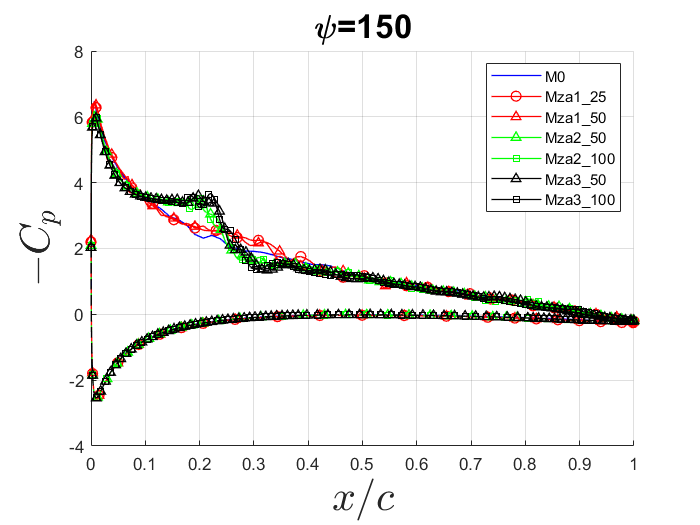
\includegraphics[width=1\textwidth]{figures/zonal_adapt_results/Cp/phase_150.png}
	\caption{ $C_p$ at $\psi$ = $150^\circ$}
	\label{fig:zonal_Cp_150}
\end{subfigure}
\begin{subfigure}[b]{0.475\textwidth}
\centering
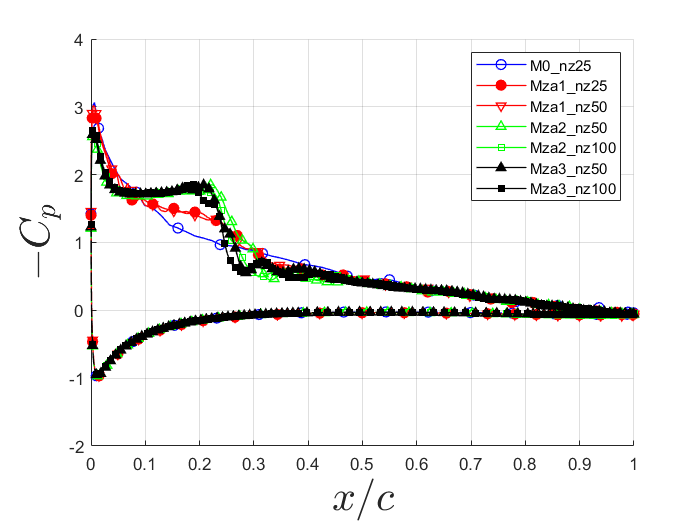
\includegraphics[width=1\textwidth]{figures/zonal_adapt_results/Cp/phase_180.png}
\caption{ $C_p$ at $\psi$ = $180^\circ$}
\label{fig:zonal_Cp_180}
\end{subfigure}
\begin{subfigure}[b]{0.475\textwidth}
\centering
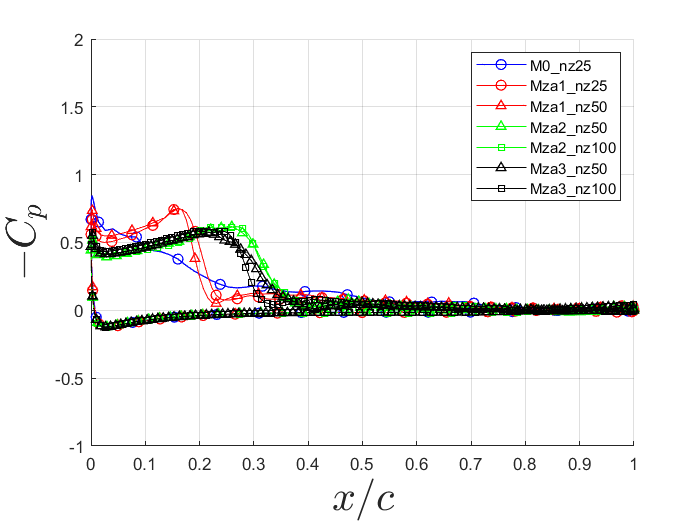
\includegraphics[width=1\textwidth]{figures/zonal_adapt_results/Cp/phase_210.png}
\caption{ $C_p$ at $\psi$ = $210^\circ$}
\label{fig:zonal_Cp_210}
\end{subfigure}
\begin{subfigure}[b]{0.475\textwidth}
\centering
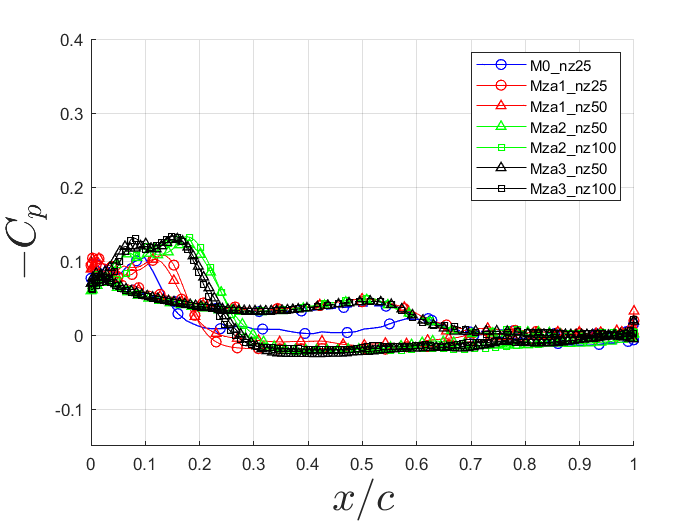
\includegraphics[width=1\textwidth]{figures/zonal_adapt_results/Cp/phase_240.png}
\caption{ $C_p$ at $\psi$ = $240^\circ$}
\label{fig:zonal_Cp_240}
\end{subfigure}
\caption{$C_p$ comparison for different meshes. Top surface $C_p$ is denoted by solid lines and bottom surface $C_p$ is denoted by dashed lines}
\label{fig:zonal_Cp_plots_LEV}
\end{figure}


\subsection{Cp: Trailing Edge Separation}


Since we have already seen through spanwise vorticity plots and Cp that the spanwise resolution of the meshes considered does not affect the solution significantly [need to figure out a better way to say this], we only show data from meshes with the second highest spanwise resolution for brevity. 
$C_p$ for phases $\psi=270^\circ$ and $\psi=300^\circ$, which is shown in Figure \ref{fig:zonal_Cp_plots_TEV}, show formation of trailing edge separation, which is evident from peaks in $C_p$ near the geometric trailing edge. 
For both these phases, $C_p$ for all meshes compare well with each other apart from M0 mesh.


\begin{figure}
\begin{subfigure}[b]{0.475\textwidth}
\centering
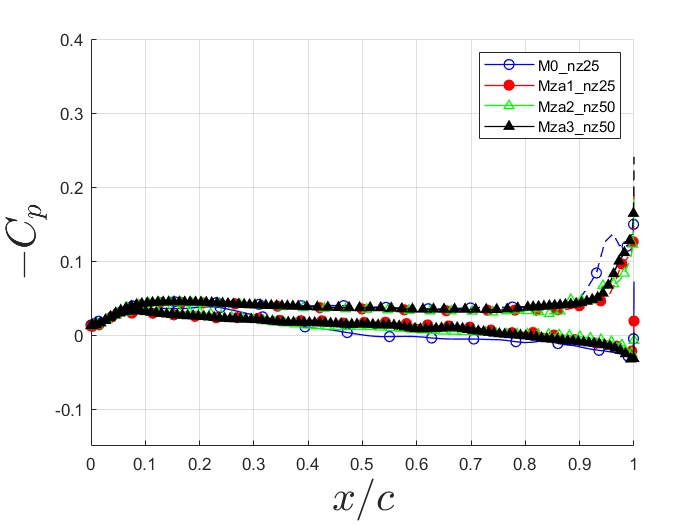
\includegraphics[width=1\textwidth]{figures/zonal_adapt_results/Cp/phase_270.png}
\caption{ $C_p$ at $\psi$ = $270^\circ$}
\label{fig:zonal_Cp_270}
\end{subfigure}
\begin{subfigure}[b]{0.475\textwidth}
\centering
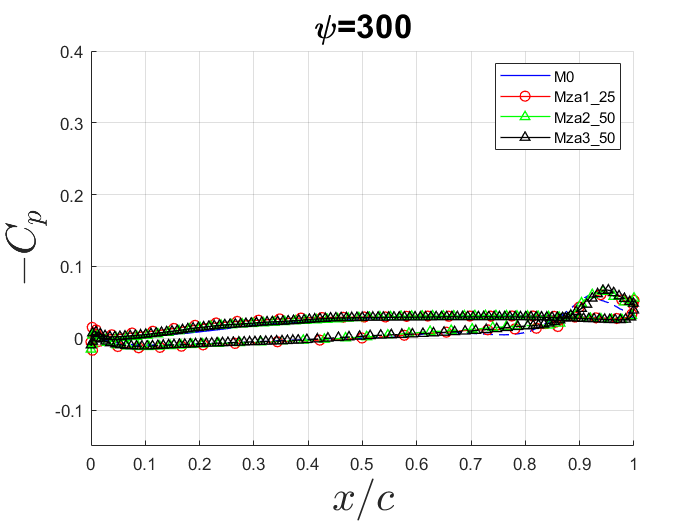
\includegraphics[width=1\textwidth]{figures/zonal_adapt_results/Cp/phase_300.png}
\caption{ $C_p$ at $\psi$ = $300^\circ$}
\label{fig:zonal_Cp_300}
\end{subfigure}
\caption{$C_p$ comparison for different meshes. Top surface $C_p$ is denoted by solid lines and bottom surface $C_p$ is denoted by dashed lines}
\label{fig:zonal_Cp_plots_TEV}
\end{figure}

